\documentclass[../thesis.tex]{subfiles}

\begin{document}

\chapter{Linking Predictive and Prescriptive Analytics for Healthcare Services}\label{chp:Linking}

\section{Introduction}
Predictive and prescriptive modelling are two powerful techniques in OR that have the ability to extract insights and guide decision-makers. Predictive models are used to forecast future outcomes based on historical data and patterns, while prescriptive models provide recommendations on how to optimise those outcomes based on certain constraints and objectives. While both techniques are valuable in their own right, they become even more powerful when linked together. By integrating predictive and prescriptive models, organisations can predict future outcomes and also make informed decisions on how to optimise those outcomes in the most effective and efficient ways possible. This can lead to more accurate and impactful decision making, and ultimately improve business and healthcare performance. The concept of linking these two methods is still relatively novel, \cite{Lopes2020,Williams2022}, especially within the healthcare field and has great potential to drive significant value for organisations across a wide range of industries.

\begin{description}
\item[\underline{Research Aim}] - This Chapter aims to link the CART results with deterministic and two-stage stochastic models together to ensure the results are consistent. It will seek to present the results in order to address the following two research objectives:
\begin{enumerate}
    \item Can linking predictive and prescriptive analytics provide improvements for decision making for frail and elderly services? - Section \ref{sec:linking}
    \item How can deterministic and two-stage stochastic models be used to plan hospital services for frail and elderly patients within Aneurin Bevan University Health Board? - Section \ref{sec:scenarioanalysis}
\end{enumerate}
\end{description}
The remainder of the Chapter is structured as follows: Section \ref{sec:linking} discusses linking the predictive and prescriptive paradigms together. Section \ref{sec:scenarioanalysis} determines the robustness of the models by applying a number of different scenarios. Section \ref{sec:generalization} discusses the flexibility within the models which allows users to apply them to other healthcare situations.

\section{Linking Paradigms}\label{sec:linking}
To investigate linking these two paradigms, two methods have been explored and applied to both the classification tree and regression tree results. The first method calculated the number of patients of each specialty and the overall average LOS for each end node. The second method used each end node and the specific LOS for each specialty and hospital within the node. These were then summed together to form the D$_{s,r}$ parameter. These two methods were run on both the regression and the classification trees, using the Microsoft Excel implementation. The results have been compared on a year-to-year basis, as well as the three year range. The VSS was calculated using the deterministic and two-stage stochastic models. For each example, a deterministic and two-stage stochastic heatmap has been provided within the Appendix \ref{app:linkeddemands}.

Using the predicted LOS from the CART models to work out demands can be more beneficial than simply using average demands due to several reasons. Firstly, predicted LOS accounts for individual patient characteristics and medical histories, allowing for more personalised estimates of resource demands, unlike average demands that treat all patients the same. Secondly, CART models can capture complex relationships between variables, resulting in more accurate predictions compared to simplistic average calculations that might overlook the impact of specific patient attributes on resource requirements. Moreover, predicted LOS adapts to changes in patient profiles and other factors affecting LOS, providing more up-to-date and flexible estimates. The model can handle outliers and extreme cases more effectively, ensuring robust capacity planning. By incorporating various patient features and clinical parameters, CART offers valuable data-driven insights into factors influencing resource demands, aiding healthcare providers in identifying areas for improvement.

\subsection{Regression Tree and Average LOS}
The first method utilised the regression tree generated in Section \ref{sec:regressiontrees} (Figure \ref{fig:finalregtree}). This tree generated 30 patient groupings determined by the 30 leaf nodes. The average LOS determined by each node was used to calculate the demand for each node. Using Equation \eqref{eq:treedemand1}, the average demand was calculated as follows:

\begin{equation}\label{eq:treedemand1}
        D_{s,r} = \sum\limits_{h \in r} D_{s,h} = \frac{\text{Number of Patients}_{s,h}*\text{Node Average LOS}}{\text{Total Number of Days in Data Set}}
\end{equation}

The procedure for calculating the average bed demand for node two is shown in Table \ref{tab:Node2Regression}. For reference, in Figure \ref{sec:regressiontrees}, node two is the second left leaf node, and it indicates if a patient meets the 11 criteria listed below:
\begin{enumerate}
    \item Admission method $\neq$ Other - transferred from another hospital
    \item Admission method $\neq$ Elective - waiting list
    \item Admission method $\neq$ Elective - booked
    \item Specialty $\neq$ Accident \& Emergency
    \item Admission method $\neq$ Elective - planned
    \item Hospital $\neq$ Ysbyty Ystrad Fawr
    \item Age Group $\neq$ 65 - 69
    \item Age Group $\neq$ 70 - 74
    \item Specialty $\neq$ Trauma \& Orthopaedic
    \item Age Group $\neq$ 75 - 79
    \item Specialty = Care Of The Elderly
\end{enumerate}

For this node, there were three hospitals included, all of which were the COTE specialty accounting for 8,776 patients. The final column of Table \ref{tab:Node2Regression} refers to the average daily bed demand across three years' worth of data. Each node's demands are consolidated for each specialty and hospital and then used for the overall demand, and are shown within Table \ref{apptab:LinkedDemands1}.
\begin{table}[h!]
    \centering\scalebox{0.8}{
    \begin{tabular}{ccccc}\toprule 
    \textbf{Hospital} & \textbf{Specialty} & \textbf{Count}& \textbf{Average LOS} & \textbf{Average Daily Demand}\\\midrule
    Nevill Hall Hospital &  Care Of The Elderly &     2696 &11.393 & 28.0251168 \\
    Royal Gwent Hospital &  Care Of The Elderly &     6076 & 11.393& 63.1604635 \\
    Ysbyty Aneurin Bevan &  Care Of The Elderly &        4 & 11.393&  0.0415803\\ \bottomrule
    \end{tabular}}
    \caption{The count of admissions and the associated average LOS for each hospital and specialty within the second node of the regression tree. The average daily bed demand has additionally been calculated.}
    \label{tab:Node2Regression}
\end{table}


Table \ref{tab:Results1} presents the results from the demands generated using the average LOS. These demands can be found within Table \ref{apptab:LinkedDemands1} in the Appendix. The same four scenarios, as listed in Table \ref{tab:scenarios1}, were applied to the demand figures. The VSS can be calculated to be 3.34\% with a saving of $\pounds$31,052.04. In comparison to Table \ref{tab:eevdettwostageresults1}, there was a difference in the deterministic solution of approximately 1.83\%, with the regression tree deploying fewer numbers of beds and nurses.
\begin{table}[h!]
    \centering\scalebox{1}{
    \begin{tabular}{cccccl}\toprule
 & \multicolumn{2}{l}{\textbf{Total Beds}} & \multicolumn{2}{c}{\textbf{Total Staff}} & \multirow{2}{*}{\textbf{Objective Function Value ($\pounds$)}}\\ \cmidrule(lr){2-3} \cmidrule(lr){4-5}
 & $x^\textnormal{bed}$           & $u^\textnormal{bed}$          & $x^\textnormal{staff}$         & $u^\textnormal{staff}$         \\ \midrule
    Deterministic      & 997 & - & 406 & - & 887,845.20 = EV \\ \midrule
    Stochastic & 836 & 359& 342 & 130 & 929,725.40 = RP \\ \midrule
    Test A & 997 & 192 & 406 & 106 &960,777.44 = EEV \\\bottomrule
    \end{tabular}}
    \caption{The EV, RP and EEV values for the $x^\textnormal{bed}$, $u^\textnormal{bed}$, $x^\textnormal{staff}$, $u^\textnormal{staff}$ decision variables and objective function using the regression tree and the average LOS across all three years.}
    \label{tab:Results1}
\end{table}

Regression tree nodes were also used to calculate the year-to-year planning to see how the model performed annually. Equation \eqref{eq:treedemand2} illustrates the process by which each annual demand was produced.
\begin{equation}\label{eq:treedemand2}
        D_{s,r,year} = \sum\limits_{h \in r} D_{s,h,year} = \frac{\text{Number of Patients}_{s,h} \times {\text{Node Average LOS}}_{year}}{\text{Number of Days in Year}}
\end{equation}
Table \ref{tab:Results2} displays the EV, RP and EEV values for each year, with the demands given in Tables \ref{apptab:LinkedDemands2a} and \ref{apptab:LinkedDemands2b}. The results reveal that the model employing the average LOS for the nodes predicted approximately the same number of beds and staff when compared to Table \ref{tab:eiveesveevdetstocresults2}. The deterministic difference, which ranged from 0.65\% to 1.13\, demonstrated that the average LOS for all three years produced results that are comparable. The locations of the bed placements can be seen within Figures \ref{fig:app1} and \ref{fig:app2}.

\begin{table}[h!]
    \centering\scalebox{0.9}{
    \begin{tabular}{ccccccl}\toprule
 & \multirow{2}{*}{\textbf{Year}}& \multicolumn{2}{l}{\textbf{Total Beds}} & \multicolumn{2}{c}{\textbf{Total Staff}} & \multirow{2}{*}{\textbf{Objective Function Value ($\pounds$)}}\\ \cmidrule(lr){3-4} \cmidrule(lr){5-6}
&& $x^\textnormal{bed}$           & $u^\textnormal{bed}$          & $x^\textnormal{staff}$         & $u^\textnormal{staff}$         \\ \midrule
     \multirow{3}{*}{Deterministic} & 2017-2018 & 1,021  & -& 386  & - & 891,125.20  =  EV$_{17-18}$ \\ 
      & 2018-2019 & 1,006 & - & 392 & - &  896,754.40 =  EV$_{18-19}$ \\
      & 2019-2020 & 997 & - & 392 & - & 883,629.40 =  EV$_{19-20}$\\ \midrule
     \multirow{3}{*}{Stochastic} & 2017-2018 & 852 & 368 & 326 & 140 & 935,847.92 =  RP$_{17-18}$ \\ 
      & 2018-2019 & 844 & 362 & 330 & 136 & 937,628.88 = RP$_{18-19}$ \\
      & 2019-2020 & 851 & 340 & 334 & 128 & 926,433.28 =  RP$_{19-20}$\\ \midrule    
     \multirow{3}{*}{Test A} & 2017-2018 & 1,021 & 192 &  386 & 104 & 965,491.36 =  EEV$_{17-18}$ \\ 
      & 2018-2019& 1,006 & 191 & 392 & 104 & 969,817.36 =  EEV$_{18-19}$ \\
      & 2019-2020 & 997 & 189 & 392 & 100 & 957,284.20 =  EEV$_{19-20}$\\ \bottomrule       
    \end{tabular}}
    \caption{The EV, RP and EEV values for the $x^\textnormal{bed}$, $u^\textnormal{bed}$, $x^\textnormal{staff}$, $u^\textnormal{staff}$ decision variables and objective function using the regression tree and the yearly average LOS.}
    \label{tab:Results2}
\end{table}

The third and final experiment has taken the average LOS for each end node and specialty, hospital and year combination. For the year 2019-2020, the total capacity had to be increased for the YAB (by 10\%), meaning additional beds would be required from other age ranges in order to meet the demand. This was due to YAB's capacity being insufficient in the UB$_{h}^{\textnormal{max, bed}}$ constraint. This would suggest the average LOS or the demand for the year 2019-2020, was larger for this hospital compared to previous years. Equation \eqref{eq:treedemand3} displays the formulation of the demands, with the overall demands listed in Tables \ref{apptab:LinkedDemands3a} and \ref{apptab:LinkedDemands3b}.

\begin{equation}\label{eq:treedemand3}
        D_{s,r,year} = \sum\limits_{h \in r} D_{s,h,year} = \frac{\text{Number of Patients}_{s,h}\times\text{Node Average LOS}_{s,h,year}}{\text{Number of Days in Year}}
\end{equation}

The results listed in Table \ref{tab:Results3} have objective function values which were comparable to those in the initial experiment. The difference in the deterministic results differs by a range of 0.72\% to 0.94\%. This highlights the possibility that by utilising the yearly node average LOS, there is little difference between the results.

\begin{table}[h!]
    \centering\scalebox{0.9}{
    \begin{tabular}{ccccccl}\toprule
 & \multirow{2}{*}{\textbf{Year}}& \multicolumn{2}{l}{\textbf{Total Beds}} & \multicolumn{2}{c}{\textbf{Total Staff}} & \multirow{2}{*}{\textbf{Objective Function Value ($\pounds$)}}\\ \cmidrule(lr){3-4} \cmidrule(lr){5-6}
&& $x^\textnormal{bed}$           & $u^\textnormal{bed}$          & $x^\textnormal{staff}$         & $u^\textnormal{staff}$         \\ \midrule
     \multirow{3}{*}{Deterministic} & 2017-2018 & 986 & - &  380 & - & 897,414.00 =  EV$_{17-18}$ \\ 
      & 2018-2019 & 1,015 & - & 392 &  - &  882,601.40 = EV$_{18-19}$ \\
      & 2019-2020 & 1,024 & - & 400 & - & 900,162.00 = EV$_{19-20}$\\ \midrule
     \multirow{3}{*}{Stochastic} & 2017-2018 & 826 &  356 & 316 &  138&  893,038.64 = RP$_{17-18}$ \\ 
      & 2018-2019 & 858 &  358 & 336& 136 & 926,218.92 = RP$_{18-19}$ \\
      & 2019-2020 & 871 & 358 & 342 & 132 & 945,905.68 = RP$_{19-20}$\\ \midrule    
     \multirow{3}{*}{Test A} & 2017-2018 & 986  & 193 & 380  & 106 &920,396.24 = EEV$_{17-18}$ \\ 
      & 2018-2019& 1,015 & 194 & 392  & 106 & 955,761.64 = EEV$_{18-19}$ \\
      & 2019-2020 & 1,024 & 198 & 400 & 106& 976,584.64 = EEV$_{19-20}$\\ \bottomrule       
    \end{tabular}}
    \caption{The EV, RP and EEV values for the $x^\textnormal{bed}$, $u^\textnormal{bed}$, $x^\textnormal{staff}$, $u^\textnormal{staff}$ decision variables and objective function using the regression tree and the yearly average LOS for each hospital and specialty.}
    \label{tab:Results3}
\end{table}



\subsection{Regression Tree and Specific LOS}
The second method also utilised the regression tree shown in Figure \ref{fig:finalregtree}. Instead of utilising the average LOS for each of the 30 end nodes, the specific LOS for each hospital and specialty inside that node was calculated. Each of the demands' generation processes are shown in Equation \eqref{eq:treedemand4}.

\begin{equation}\label{eq:treedemand4}
        D_{s,r} = \sum\limits_{h \in r} D_{s,h} = \frac{\text{Number of Patients}_{s,h}\times{\text{Specific LOS}_{s,h}}}{1096}
\end{equation}

Table \ref{tab:Node2Regressionb} presents the second node within the regression tree and determines how each of the demands was produced within this node. These findings demonstrated that employing particular hospital and specialty LOS, increased the demand for beds overall in RGH by one bed when compared to Table \ref{tab:Node2Regression}. The generated demands can be viewed in Table \ref{apptab:LinkedDemands4}.

\begin{table}[h!]
    \centering\scalebox{0.8}{
    \begin{tabular}{ccccc}\toprule 
    \textbf{Hospital} & \textbf{Specialty} & \textbf{Count}& \textbf{Specific LOS} & \textbf{Average Daily Demand}\\\midrule
    Nevill Hall Hospital &  Care Of The Elderly &     2696 &11.412 & 28.0729927 \\
    Royal Gwent Hospital &  Care Of The Elderly &     6076 & 11.554& 64.0510949 \\
    Ysbyty Aneurin Bevan &  Care Of The Elderly &        4 & 6.250&  0.0228102\\ \bottomrule
    \end{tabular}}
    \caption{The count of admissions and the associated specific LOS for each hospital and specialty within the second node of the regression tree. The average daily bed demand has additionally been calculated.}
    \label{tab:Node2Regressionb}
\end{table}

The findings for the deterministic and two-stage stochastic models are shown in Table \ref{tab:Results4}, with the EEV also being calculated to determine the VSS.

\begin{table}[h!]
    \centering
    \begin{tabular}{cccccl}\toprule
 & \multicolumn{2}{l}{\textbf{Total Beds}} & \multicolumn{2}{c}{\textbf{Total Staff}} & \multirow{2}{*}{\textbf{Objective Function Value ($\pounds$)}}\\ \cmidrule(lr){2-3} \cmidrule(lr){4-5}
 & $x^\textnormal{bed}$           & $u^\textnormal{bed}$          & $x^\textnormal{staff}$         & $u^\textnormal{staff}$         \\ \midrule
    Deterministic      & 1,011 & - & 388 & - & 889,242.60 = EV \\ \midrule
    Stochastic &842&361 & 320 & 134&  925,599.36 = RP \\ \midrule
    Test A & 1,011 & 186 & 579 & 94 & 958,630.76 = EEV \\\bottomrule
    \end{tabular}
    \caption{The EV, RP and EEV values for the $x^\textnormal{bed}$, $u^\textnormal{bed}$, $x^\textnormal{staff}$, $u^\textnormal{staff}$ decision variables and objective function using the regression tree and the specific LOS across all three years.}
    \label{tab:Results4}
\end{table}
The specific LOS model had lower deterministic and two-stage stochastic objective values as compared to the regression tree with average LOS findings. This shows that if the exact LOS was used, rather than node averages, additional cost savings would be produced. The VSS produced a saving of $\pounds$33,031.40 per day (3.57\%). The specific LOS generated from each regression tree node could be used to analyse these results on an annual basis (Tables \ref{apptab:LinkedDemands5a} and \ref{apptab:LinkedDemands5b}). To calculate the demands for each specialty and region for each year, Equation \eqref{eq:treedemand5} could be applied.

\begin{equation}\label{eq:treedemand5}
        D_{s,r,year} = \sum\limits_{h \in r} D_{s,h,year} = \frac{\text{Number of Patients}_{s,h}\times{\text{Specific LOS}_{s,h,year}}}{{\text{Number of Days in Year}}}
\end{equation}

Table \ref{tab:Results5} presents the results after the tool had optimised the bed and staffing numbers based on the demand values. The number of staff deployed in the first two years remained constant before reducing in the third year. Each year saw a reduction in the EV overall. The VSS ranged from 3.28\% to 3.45\%, once more demonstrating the advantages of employing the stochastic approach.

\begin{table}[h!]
    \centering\scalebox{0.9}{
    \begin{tabular}{ccccccl}\toprule
 & \multirow{2}{*}{\textbf{Year}}& \multicolumn{2}{l}{\textbf{Total Beds}} & \multicolumn{2}{c}{\textbf{Total Staff}} & \multirow{2}{*}{\textbf{Objective Function Value ($\pounds$)}}\\ \cmidrule(lr){3-4} \cmidrule(lr){5-6}
&& $x^\textnormal{bed}$           & $u^\textnormal{bed}$          & $x^\textnormal{staff}$         & $u^\textnormal{staff}$         \\ \midrule   \multirow{3}{*}{Deterministic} & 2017-2018 & 1,009 & - & 370 & - & 874,693.00 = EV$_{17-18}$ \\ 
      & 2018-2019 & 998 & - & 370 & - & 873,709.00 = EV$_{18-19}$ \\
      & 2019-2020 &  988 & - & 364 & -& 869,959.80 = EV$_{19-20}$\\\midrule
     \multirow{3}{*}{Stochastic} & 2017-2018 & 839 & 369 & 310 & 132 & 917,423.68 = RP$_{17-18}$ \\ 
      & 2018-2019 & 832 & 363 & 308 & 132 & 914,315.56 = RP$_{18-19}$ \\
      & 2019-2020 & 838  & 344  & 310 & 130 & 911,420.56 = RP$_{19-20}$\\ \midrule
      \multirow{3}{*}{Test A}& 2017-2018 & 1,009 & 194 & 370 & 100 & 947,517.00 = EEV$_{17-18}$\\
      & 2018-2019 & 998 & 189 & 370 & 100 & 945,583.80 = EEV$_{18-19}$\\
& 2019-2020 & 988 & 189 & 364 & 100 & 942,856.60 = EEV$_{19-20}$\\\bottomrule      
    \end{tabular}}
    \caption{The EV, RP and EEV values for the $x^\textnormal{bed}$, $u^\textnormal{bed}$, $x^\textnormal{staff}$, $u^\textnormal{staff}$ decision variables and objective function using the regression tree and the yearly specific LOS.}
    \label{tab:Results5}
\end{table}

\subsection{Classification Tree and Average LOS}
The third method utilised the classification tree displayed by Figure \ref{fig:finalclasstree}. The classification tree yielded 30 patient groupings, with patients falling into one of two categories. Recall Equation \eqref{eq:treedemand1} to create demands and to calculate the D$_{s,r}$ variable:

\begin{equation}
        D_{s,r} = \sum\limits_{h \in r} D_{s,h} = \frac{\text{Number of Patients}_{s,h}\times\text{Node Average LOS}}{1096} \tag{\ref{eq:treedemand1} revisited}\\
\end{equation}

For patients who fell into a `$<$1' node, meant the majority of patients were discharged on the same day they were admitted. In spite of this, there were certain patients in every case who were put in this category despite not meeting the criteria. As a result, to take these individuals into consideration, the average LOS would not be zero days.

If a patient fulfilled all seven of the following criteria, they were grouped into the ninth node of the CART tree.
\begin{enumerate}
    \item Admission method = Elective - waiting list
    \item Specialty $\neq$ Trauma \& Orthopaedic
    \item Specialty $\neq$ General Surgery
    \item Specialty $\neq$ Urology
    \item Specialty $\neq$ Ear, Nose \& Throat
    \item Specialty $\neq$ Gynaecology
    \item Specialty = Respiratory
\end{enumerate}

For this node, the majority of patients were grouped into the `$<$1' category, and the average LOS was less than one (0.913918 days). The average daily demand required for each specialty and hospital inside this node may subsequently be determined using this value (Table \ref{tab:classnodeexample}). The associated demands are presented in Table \ref{apptab:LinkedDemands6}, within the Appendix.

\begin{table}[h!]
    \centering\scalebox{0.8}{
    \begin{tabular}{ccccc}\toprule
        \textbf{Hospital} & \textbf{Specialty} & \textbf{Count} & \textbf{Average LOS} & \textbf{Average Daily Demand}  \\\midrule
         Nevill Hall Hospital & Respiratory &   690 & 0.913918 & 0.575368 \\
         Royal Gwent Hospital & Respiratory &   553 &0.913918 & 0.461128 \\ \bottomrule
    \end{tabular}}
    \caption{The count of admissions and the associated average LOS for each hospital and specialty within the ninth node of the classification tree. The average daily bed demand has additionally been calculated.}
    \label{tab:classnodeexample}
\end{table}

The results using these demands are shown in Table \ref{tab:Results6}. By deploying 1,015 beds and 428 nurses, an EV value of $\pounds$826,712.60 was produced. Similar to prior findings, fewer beds were used than the averages produced in Chapter \ref{chp:Experimental Analysis}. A significant reduction in the total objective function resulted from the deployment of beds to different hospital locations. The location of these beds can be seen in Figure \ref{fig:app14a} in the Appendix.


\begin{table}[h!]
    \centering
    \begin{tabular}{cccccl}\toprule
 & \multicolumn{2}{l}{\textbf{Total Beds}} & \multicolumn{2}{c}{\textbf{Total Staff}} & \multirow{2}{*}{\textbf{Objective Function Value ($\pounds$)}}\\ \cmidrule(lr){2-3} \cmidrule(lr){4-5}
 & $x^\textnormal{bed}$           & $u^\textnormal{bed}$          & $x^\textnormal{staff}$         & $u^\textnormal{staff}$         \\ \midrule
    Deterministic      & 1,015 & - & 428 & - & 826,712.60 = EV \\ \midrule
    Stochastic & 862 & 352 & 360&138 &  866,576.52 = RP \\ \midrule
    Test A & 1,015  & 190 & 428 & 102 & 892,880.68 = EEV \\\bottomrule
    \end{tabular}
    \caption{The EV, RP and EEV values for the $x^\textnormal{bed}$, $u^\textnormal{bed}$, $x^\textnormal{staff}$, $u^\textnormal{staff}$ decision
variables and objective function using the classification tree and the average LOS across all three years.}
    \label{tab:Results6}
\end{table}

The VSS was calculated to be 3.04\%, demonstrating that there is a difference between the two models using this strategy even when classification trees are used to generate the demand. In comparison to the earlier models, the results used a similar number of beds, but the objective values were much lower. One explanation for this would be that fewer beds were deployed in the more expensive units because their LOS's were shorter and their daily demands are consequently lower.

Equation \eqref{eq:treedemand2} described how each of the demands was calculated after further analysis on a year-to-year basis. The formulated demand was inputted into the deterministic and two-stage stochastic models, (Tables \ref{apptab:LinkedDemands7a} and \ref{apptab:LinkedDemands7b}) after being summed up across each node.

\begin{equation}
        D_{s,r,year} = \sum\limits_{h \in r} D_{s,h,year} = \frac{\text{Number of Patients}_{s,h} \times {\text{Node Average LOS}}_{year}}{\text{Number of Days in Year}} \tag{\ref{eq:treedemand2} revisited}
\end{equation}

The EV, RP, and EEV values are shown in Table \ref{tab:Results7}, demonstrating how the objective value fluctuates from year-to-year. Although using a comparable number of beds as in the prior experiment, the objective values obtained are lower. Figures \ref{fig:app15a} - \ref{fig:app17b} show where these beds are located. The two-stage stochastic model's advantage is demonstrated by the VSS, which varies from 3.11\% to 3.35\%. These findings demonstrate the advantages of yearly planning as opposed to preparing in three year increments.

\begin{table}[h!]
    \centering\scalebox{0.9}{
    \begin{tabular}{ccccccl}\toprule
 & \multirow{2}{*}{\textbf{Year}}& \multicolumn{2}{l}{\textbf{Total Beds}} & \multicolumn{2}{c}{\textbf{Total Staff}} & \multirow{2}{*}{\textbf{Objective Function Value ($\pounds$)}}\\ \cmidrule(lr){3-4} \cmidrule(lr){5-6}
&& $x^\textnormal{bed}$           & $u^\textnormal{bed}$          & $x^\textnormal{staff}$         & $u^\textnormal{staff}$         \\ \midrule
      \multirow{3}{*}{Deterministic} & 2017-2018 & 979  & - & 390 & - & 805,452.00 =  EV$_{17-18}$ \\ 
       & 2018-2019 & 1,002 & - &  398 & - & 834,264.60  =  EV$_{18-19}$ \\
       & 2019-2020 &  1,005 & - & 404 & - & 842,867.80 =  EV$_{19-20}$\\ \midrule
      \multirow{3}{*}{Stochastic} & 2017-2018 & 819 & 350 &324  & 136 &  843,654.48 =  RP$_{17-18}$ \\ 
       & 2018-2019 & 844  &  359 & 338 & 140 & 875,908.56 = RP$_{18-19}$ \\
       & 2019-2020 & 842 & 363 & 346 & 134 & 882,667.16 = RP$_{19-20}$\\ \midrule    
      \multirow{3}{*}{Test A} & 2017-2018 & 979 & 184 & 390  &92  & 869,933.28 = EEV$_{17-18}$ \\ 
       & 2018-2019& 1,002 & 193 & 398  & 106 & 904,084.84 = EEV$_{18-19}$ \\
       & 2019-2020 & 1,005 & 194 & 404 &  96&  912,268.44 = EEV$_{19-20}$\\ \bottomrule       
    \end{tabular}}
    \caption{The EV, RP and EEV values for the $x^\textnormal{bed}$, $u^\textnormal{bed}$, $x^\textnormal{staff}$, $u^\textnormal{staff}$ decision
variables and objective function using the classification tree and the yearly average LOS.}
    \label{tab:Results7}
\end{table}

Instead of utilising the node average for the model, these results were expanded to include the average LOS per year. This applied Equation \eqref{eq:treedemand3} to calculate the demands for the model and the results can be seen in Tables \ref{apptab:LinkedDemands8a} and \ref{apptab:LinkedDemands8b}. By employing this technique, it ensured that specialty LOS was taken into consideration, particularly for specialties which have longer LOS's.

\begin{equation}
        D_{s,r,year} = \sum\limits_{h \in r} D_{s,h,year} = \frac{\text{Number of Patients}_{s,h}\times\text{Node Average LOS}_{s,h,year}}{\text{Number of Days in Year}} \tag{\ref{eq:treedemand3} revisited}
\end{equation}

The results are presented within Table \ref{tab:Results8}, and graphically illustrated in Figures \ref{fig:app18a} - 
 \ref{fig:app20b} in the Appendix. The results show that more beds and nurses were deployed in 2017–2018 when compared against using the average node LOS. The objective value was lower from 2018, as fewer beds and nurses were being deployed.

\begin{table}[h!]
    \centering\scalebox{0.9}{
    \begin{tabular}{ccccccl}\toprule
 & \multirow{2}{*}{\textbf{Year}}& \multicolumn{2}{l}{\textbf{Total Beds}} & \multicolumn{2}{c}{\textbf{Total Staff}} & \multirow{2}{*}{\textbf{Objective Function Value ($\pounds$)}}\\ \cmidrule(lr){3-4} \cmidrule(lr){5-6}
&& $x^\textnormal{bed}$           & $u^\textnormal{bed}$          & $x^\textnormal{staff}$         & $u^\textnormal{staff}$         \\ \midrule
      \multirow{3}{*}{Deterministic} & 2017-2018 & 993  & - &  398 & - & 815,342.60 =  EV$_{17-18}$ \\ 
       & 2018-2019 & 993& - & 398 & - & 829,485.60 =  EV$_{18-19}$ \\
       & 2019-2020 &  995 & - & 400 & - & 837,880.00  =  EV$_{19-20}$\\ \midrule
      \multirow{3}{*}{Stochastic} & 2017-2018 & 832 & 359 & 330 & 140 & 856,341.72  = RP$_{17-18}$ \\ 
       & 2018-2019 &  838 & 352 & 338  & 140 & 870,815.16 =  RP$_{18-19}$ \\
       & 2019-2020 & 830 & 363 & 340 & 140 &  878,140.24 =  RP$_{19-20}$\\ \midrule    
      \multirow{3}{*}{Test A} & 2017-2018 & 993  & 192 &  398  & 100 & 883,441 = EEV$_{17-18}$ \\ 
     & 2018-2019 & 993  & 191 &  398  & 104 & 899,117.12 = EEV$_{17-18}$ \\ 
       & 2019-2020 & 995 & 192 & 400 & 102 & 907,630.08 = EEV$_{19-20}$\\ \bottomrule       
    \end{tabular}}
    \caption{The EV, RP and EEV values for the $x^\textnormal{bed}$, $u^\textnormal{bed}$, $x^\textnormal{staff}$, $u^\textnormal{staff}$ decision variables and objective function using the classification tree and the yearly average LOS for each hospital and specialty.}
    \label{tab:Results8}
\end{table}


\subsection{Classification Tree and Specific LOS}
The classification tree depicted in Figure \ref{fig:finalclasstree} was used by the fourth and final method. Instead of utilising the average LOS for each of the 30 end nodes, the LOS was calculated for each hospital and specialty inside that node. The generation of each demand is shown in Equation \eqref{eq:treedemand4}.

\begin{equation}
        D_{s,r} = \sum\limits_{h \in r} D_{s,h} = \frac{\text{Number of Patients}_{s,h}\times{\text{Specific LOS}_{s,h}}}{1096} \tag{\ref{eq:treedemand4} revisited}
\end{equation}

Table \ref{tab:Node2Regressiond} presents the ninth node within the classification tree and determines how each of the demands was generated within this node. These results in comparison with Table \ref{tab:classnodeexample}, have shown that using specific hospital and specialty, LOS overall did not increase the number of beds required in this node. The generated demands can be viewed in Table \ref{apptab:LinkedDemands9}. At the deterministic stage, the required number of beds decreased across all nodes from 1,015 beds to 1,011 beds (Table \ref{tab:Results9}). 

\begin{table}[h!]
    \centering\scalebox{0.8}{
    \begin{tabular}{ccccc}\toprule 
    \textbf{Hospital} & \textbf{Specialty} & \textbf{Count}& \textbf{Average LOS} & \textbf{Average Daily Demand}\\\midrule
    Nevill Hall Hospital &  Respiratory &     690 &0.531884 & 0.3348540 \\
    Royal Gwent Hospital &  Respiratory &     553 & 1.39057& 0.7016423 \\ \bottomrule
    \end{tabular}}
    \caption{The count of admissions and the associated specific LOS for each hospital and specialty within the ninth node of the classification tree. The average daily bed demand has additionally been calculated.}
    \label{tab:Node2Regressiond}
\end{table}

Table \ref{tab:Results9} presents the results for the deterministic and two-stage stochastic model, with the EEV also being calculated to determine the VSS.

\begin{table}[h!]
    \centering
    \begin{tabular}{cccccl}\toprule
 & \multicolumn{2}{l}{\textbf{Total Beds}} & \multicolumn{2}{c}{\textbf{Total Staff}} & \multirow{2}{*}{\textbf{Objective Function Value ($\pounds$)}}\\ \cmidrule(lr){2-3} \cmidrule(lr){4-5}
 & $x^\textnormal{bed}$           & $u^\textnormal{bed}$          & $x^\textnormal{staff}$         & $u^\textnormal{staff}$         \\ \midrule
    Deterministic      &  1,011 & - &388  & - & 889,242.60 = EV \\ \midrule
    Stochastic & 842 & 361 & 320 & 134 & 925,599.36 = RP \\ \midrule
    Test A & 1,011& 186 & 388 & 94 & 958,624.36 = EEV \\\bottomrule
    \end{tabular}
    \caption{The EV, RP and EEV values for the $x^\textnormal{bed}$, $u^\textnormal{bed}$, $x^\textnormal{staff}$, $u^\textnormal{staff}$ decision variables and objective function using the classification tree and the specific LOS across all three years.}
    \label{tab:Results9}
\end{table}

Comparing to the regression tree with average LOS results, the deterministic and two-stage stochastic objective values were higher in the specific LOS model. This suggested that using node averages might not produce sufficient capacity for beds and staff. The VSS produced a saving of $\pounds$21,344.72 per day (2.09\%). 

The individual LOS generated from each regression tree node could be used to analyse these results on an annual basis (Tables \ref{apptab:LinkedDemands10a} and \ref{apptab:LinkedDemands10b}). Equation \eqref{eq:treedemand5} was used to determine the demands for each specialty and region for each year.

\begin{equation}
        D_{s,r,year} = \sum\limits_{h \in r} D_{s,h,year} = \frac{\text{Number of Patients}_{s,h}\times{\text{Specific LOS}_{s,h,year}}}{{\text{Number of Days in Year}}} \tag{\ref{eq:treedemand5} revisited}
\end{equation}

The results have shown that the model optimised the bed and staff numbers based on the demand data, as shown in Table \ref{tab:Results5}. Over time the number of beds and nurses deployed has declined. Although more beds are deployed in the first year, the second and third years have larger objective values due to different specialty beds being deployed.

\begin{table}[h!]
    \centering\scalebox{0.9}{
    \begin{tabular}{ccccccl}\toprule
 & \multirow{2}{*}{\textbf{Year}}& \multicolumn{2}{l}{\textbf{Total Beds}} & \multicolumn{2}{c}{\textbf{Total Staff}} & \multirow{2}{*}{\textbf{Objective Function Value ($\pounds$)}}\\ \cmidrule(lr){3-4} \cmidrule(lr){5-6}
&& $x^\textnormal{bed}$           & $u^\textnormal{bed}$          & $x^\textnormal{staff}$         & $u^\textnormal{staff}$         \\ \midrule
     \multirow{3}{*}{Deterministic} & 2017-2018 & 1,007 & - & 388 & - & 869,740.60 = EV$_{17-18}$ \\ 
      & 2018-2019 & 1,004 & - & 386 & - & 875,147.20 = EV$_{18-19}$ \\
      & 2019-2020 & 1,000 & - & 380 & - & 877,707.00 = EV$_{19-20}$\\\midrule
     \multirow{3}{*}{Stochastic} & 2017-2018 & 836 & 367 & 318 & 136  & 911,555.20 = RP$_{17-18}$ \\ 
      & 2018-2019 & 839 & 367 & 320 & 138 & 917,521.08  = RP$_{18-19}$ \\
      & 2019-2020 &848 & 351 & 328 & 136 & 922,334.40 = RP$_{19-20}$\\ \midrule
      \multirow{3}{*}{Test A}& 2017-2018 & 1,007 & 193  & 388 & 100 &  941,426.60 = EEV$_{17-18}$\\
      & 2018-2019 & 1,004 & 192 &  386 & 106 & 948,915.04 = EEV$_{18-19}$\\
      & 2019-2020 & 1,000  & 193 & 380 & 104 &952,017.56 = EEV$_{19-20}$\\\bottomrule      
    \end{tabular}}
    \caption{The EV, RP and EEV values for the $x^\textnormal{bed}$, $u^\textnormal{bed}$, $x^\textnormal{staff}$, $u^\textnormal{staff}$ decision variables and objective function using the classification tree and the yearly specific LOS.}
    \label{tab:Results5}
\end{table}

\section{Scenario Analysis}\label{sec:scenarioanalysis}
Scenario analysis is a powerful tool used in strategic planning and decision making. It involves developing and examining a variety of hypothetical future scenarios in order to understand their potential effects on a given situation or system. This approach allows decision-makers to investigate a range of possible outcomes and uncertainties, which can be used to develop their strategies and plans. Scenario analysis typically involves identifying the key drivers of change and uncertainty in a particular situation or system. These drivers can include economic trends, technological developments, political factors, and social changes. Following the identification of these drivers, various scenarios are created by taking into account how they could interact and change over time. The resulting scenarios provide decision-makers with a range of plausible futures to consider, each with its own set of opportunities and challenges. By exploring these various scenarios, decision-makers can better understand the risks and opportunities associated with different strategies and plans, and make more informed decisions about how to proceed.

This section will utilise the CART models to feed into the deterministic and two-stage stochastic models. The underlying assumption with predictive models is that the patterns observed in the historical data will continue to hold in the future under similar circumstances. This might be particularly challenging in healthcare, particularly for predicting LOS in hospitals. Moreover, historical data used for training the predictive models may include instances of poor system performance or inefficiencies that could impact the generalisability of the model's predictions to future scenarios.

When using a point estimate (i.e. average) for predicting hospital LOS, typically the mean LOS is calculated across the entire data set. This single average value is then used as the prediction for all patients, regardless of their individual characteristics. Consequently, this approach does not account for the diversity of patients, medical conditions, and other factors that contribute to variations. By utilising CART, patient subgroups based on characteristics are created and subgroup specific average LOS values for predictions are created. This approach recognises the diversity in patient profiles and medical conditions, providing more variation in the demand values.

This section aims to utilise the methods of linking the predictive and prescriptive models and apply a variety of scenarios to them. Specific scenarios in ABUHB have been identified through collaboration with senior staff within the health board. The health board raised four main concerns regarding future changes and how this may impact bed and staffing requirements. These were as follows:

\begin{enumerate}
    \item Addition of a new hospital
    \item What if demand cannot be met? 
    \item Re-evaluating the current setup
    \item Long-term predictions
\end{enumerate}

The remainder of this section will discuss each of the above points.

\subsection{Addition of a New Hospital}\label{sec:scenario1}
The Grange University Hospital (GUH), a new hospital with a focus on critical care, opened within the health board in November 2020 with the goal of treating the most seriously ill patients or those with significant injuries. It also serves as the designated trauma centre for the area \cite{NHSWalesa}. The hospital opened with 560 beds and features a 24 hours acute assessment unit, A\&E unit and provides 24/7 emergency care for patients that need specialist and critical care. To help alleviate the strains brought on by the second wave of Covid-19 and winter seasonal stresses, GUH opened earlier than its planned date of March 2021. The hospital was designed to treat patients who cannot be safely managed at one of the local general hospitals, and as such required specialties to be relocated throughout the health board. As of 2022, GUH catered for 18 specialties and as a result the number of specialties offered by other hospitals was reduced. In total, the number of specialties locations offered by the hospitals reduced from 98 to 92. An updated visual of specialty and hospital locations can be seen within Figure \ref{fig:relocation}.
\begin{figure}[h!]
    \centering
    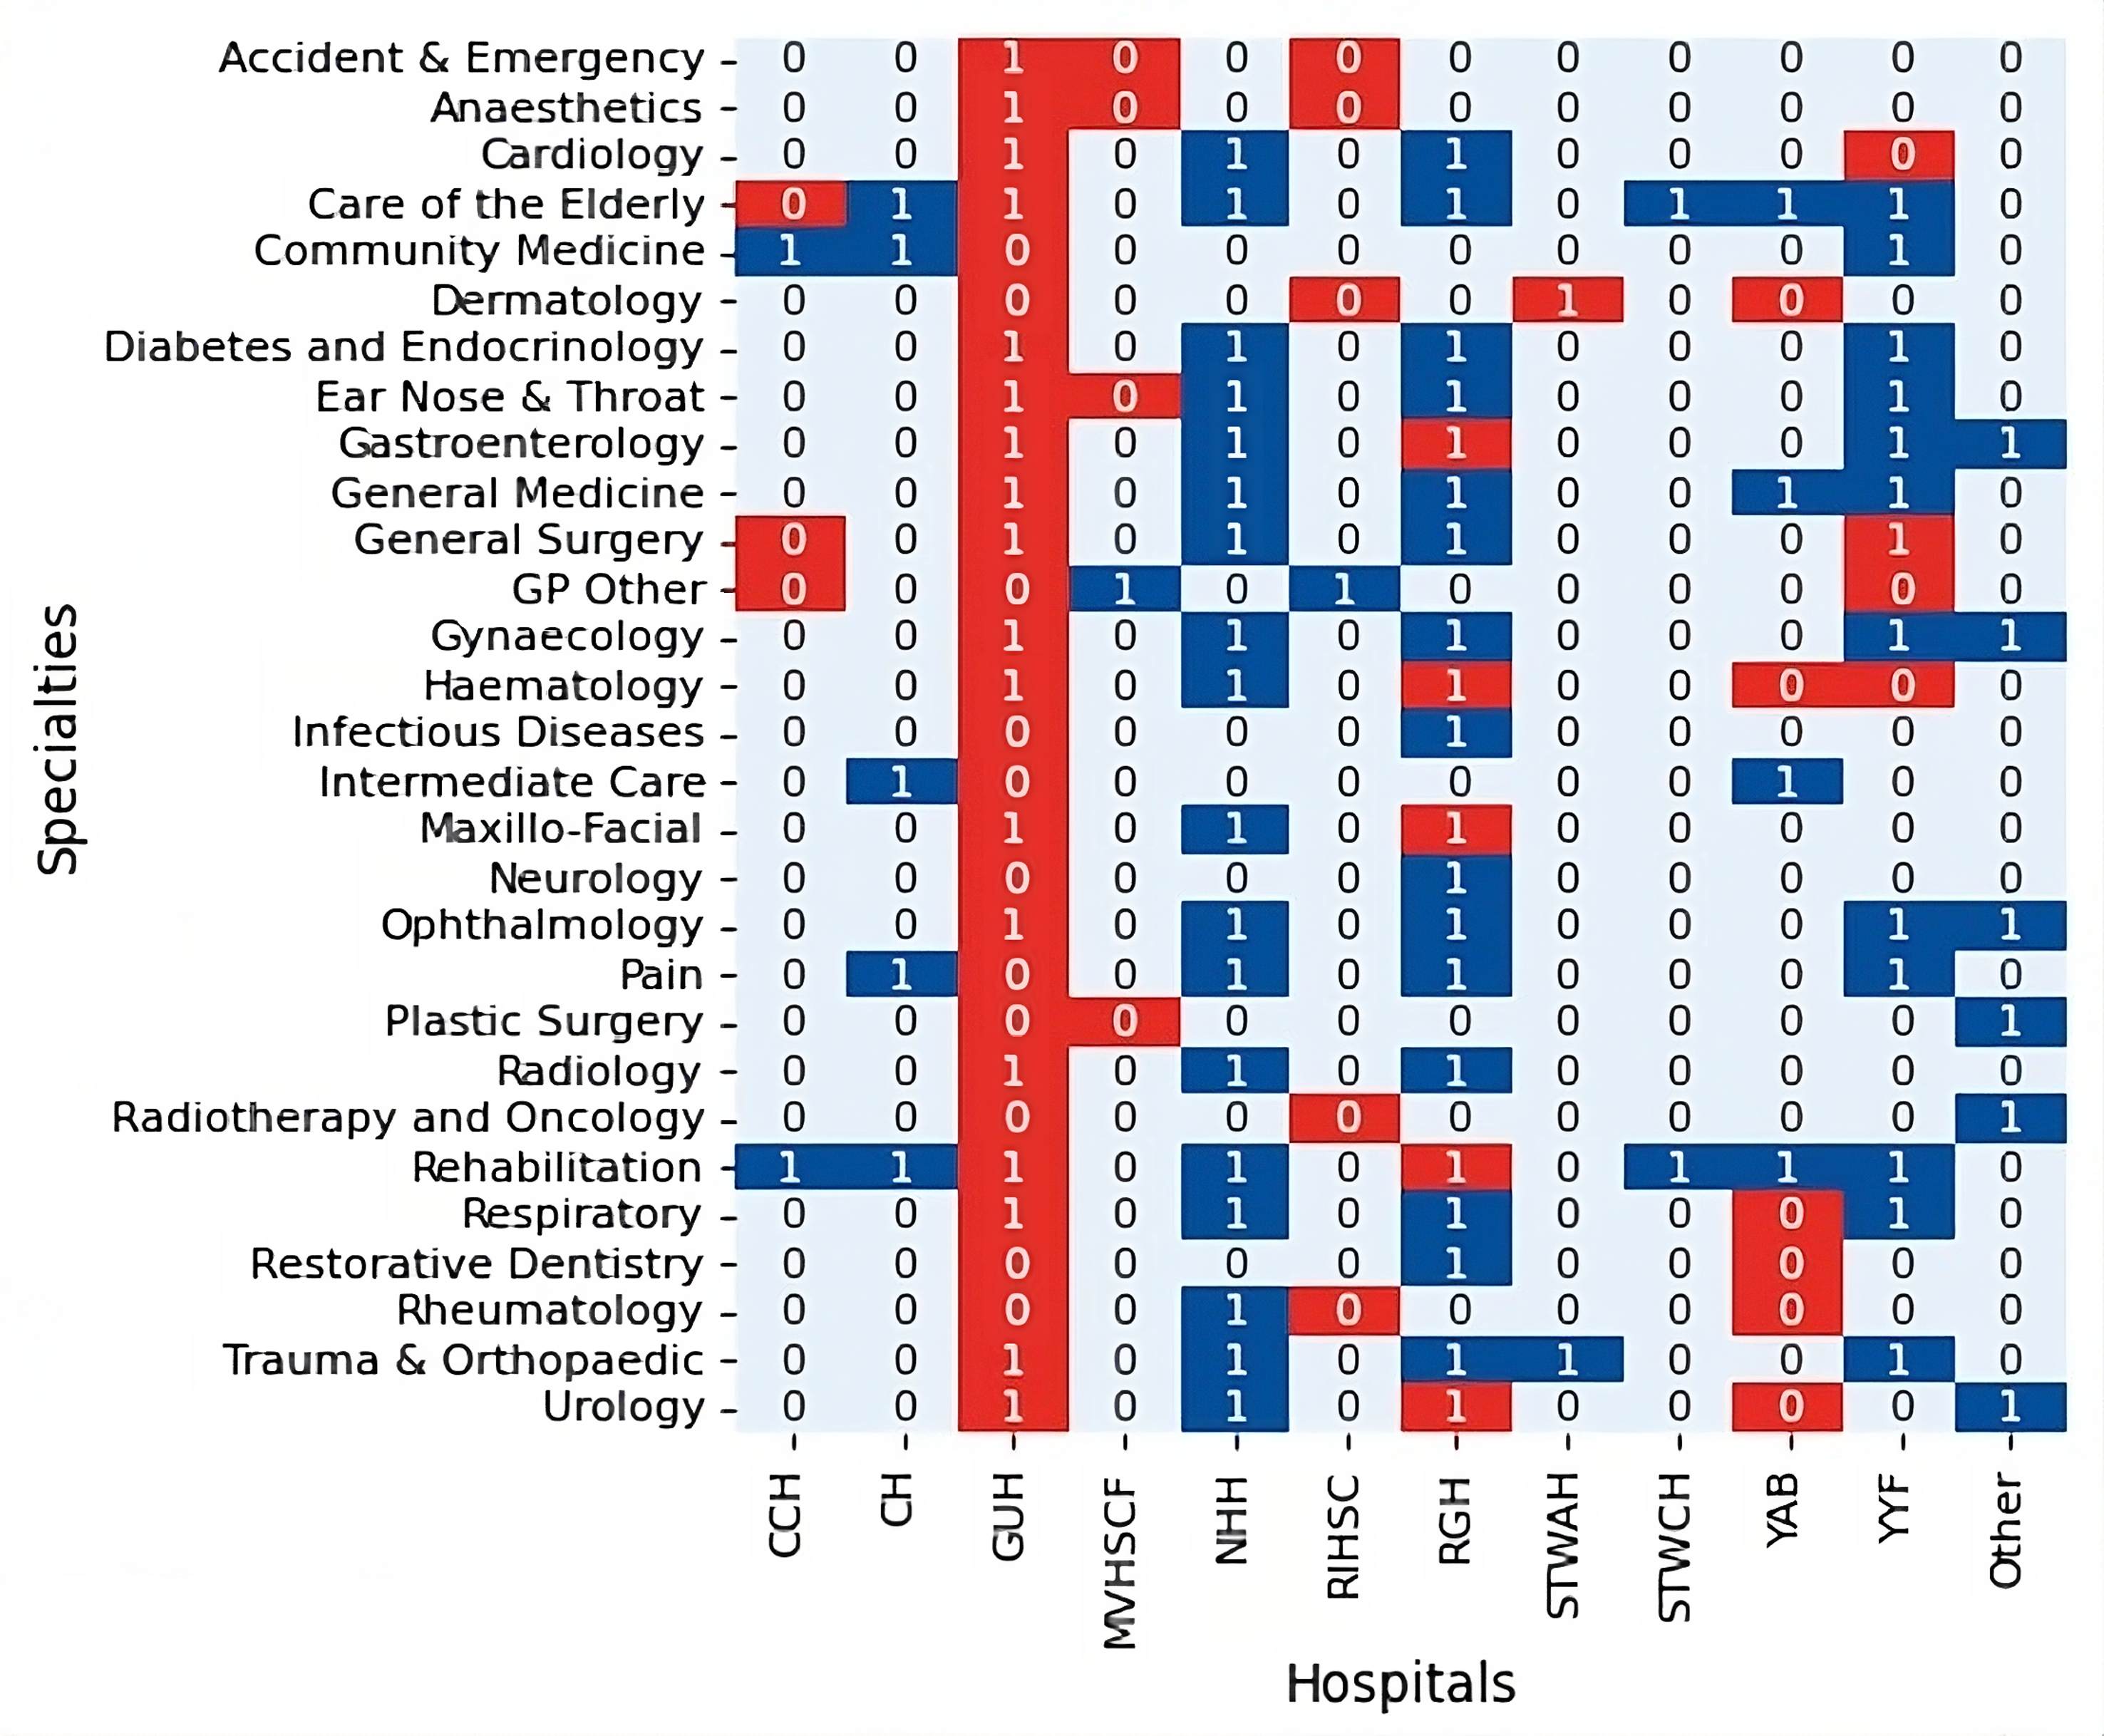
\includegraphics[scale=0.12]{Chapters/Chapter6/Figures/UpdatedSpec-transformed.png}
    \caption{An updated version of the hospitals and specialties in ABUHB, with a `1' indicating a specialty is present in a given hospital. For cells with a \textcolor{red}{red} background, displays where specialties have opened or closed since the opening of the Grange University Hospital (GUH).}
    \label{fig:relocation}
\end{figure}


In order to incorporate GUH into the model with the existing data, the assumption has been made that patients will be admitted to any hospital within the health board and the regional restrictions are lifted. This results in the following constraints, where the $D_{s,r}$ parameter is changed to $D_{s}$:\\
\underline{Deterministic Model}
\begin{equation}
    \sum_{h\in\mathcal{H}} x^\textnormal{bed}_{s,h}\geq D_{s}  \hspace{0.5cm} \forall  s \in \mathcal{S}
\end{equation}
\underline{Two-Stage Stochastic Model}
\begin{equation}
    \sum_{h\in\mathcal{H}} x^\textnormal{bed}_{s,h} +  \sum_{h\in\mathcal{H}} u^\textnormal{bed}_{s,h,k} \geq D_{s,k} \hspace{0.5cm} \forall s \in \mathcal{S}, k \in \mathcal{K}\\
\end{equation}

The cost for each Welsh specialty bed was calculated using open source data from Public Health Scotland. The specialty average for the Welsh-generated data was the same as the specialty average for the Scottish-generated data, and the Welsh data also fell within the specified range of the Scottish-generated data. In order to match the average of the Scottish data, new values had to be constructed because the numbers were originally created using the prior hospital/specialty location possibilities without taking GUH into account. If a specialty remains in the same hospital, the previous cost will remain the same. Nonetheless, in some circumstances, hospitals no longer offer as many specialties as they once did, falling short of the Scottish average. As a result, these values are altered to conform to the average. Similarly, since the opening of GUH, the number of available beds within existing hospitals has decreased. GUH has 560 beds within the hospital available to all patients, however, the number has been scaled down to 300 to take the age group into consideration. Because fewer beds are available, this has an impact on the K$_{s,h}$, UB$^\textnormal{max, bed, 1st}_{h}$ and UB$^\textnormal{max, bed, 2nd}_{h}$ variables.

To demonstrate how the model would perform with the addition of GUH and the relaxation of the regional demand constraint, the regression tree with the specific LOS over three years' worth of data will be utilised (Table \ref{apptab:LinkedDemands4} within the Appendix). The model utilised the three scenarios previously discussed, where demand remains constant, increases by 20\% and decreases by 20\%, all with equal probabilities of a third. The deterministic model yielded an objective value of $\pounds669,699.20$ with the deployment of 982 beds and 326 nursing staff (Table \ref{tab:Scenario1Results}). In the case of the two-stage stochastic model, this amount rises to $\pounds$686,198.04. These findings demonstrate that establishing GUH and redesigning the specialties within hospitals resulted in a difference of approximately $\pounds$200,000.00. This shows the benefit to decision-makers of opening this hospital, and the potential savings if the ABUHB costings resembled those of the NHS Scotland data. The VSS is calculated to be 5.20\% demonstrating the benefits of utilising the two-stage stochastic model over the traditional deterministic model.

\begin{table}[h!]
    \centering
    \begin{tabular}{cccccl}\toprule
 & \multicolumn{2}{l}{\textbf{Total Beds}} & \multicolumn{2}{c}{\textbf{Total Staff}} & \multirow{2}{*}{\textbf{Objective Function Value ($\pounds$)}}\\ \cmidrule(lr){2-3} \cmidrule(lr){4-5}
          & $x^\textnormal{bed}$           & $u^\textnormal{bed}$          & $x^\textnormal{staff}$         & $u^\textnormal{staff}$         \\ \midrule
 Deterministic & 982 & - & 326 & - & $\pounds$669,699.20 = EV \\
 Stochastic & 817 & 399 & 268 & 120 & $\pounds$686,198.04 = RP \\
 Test A & 982 & 188 & 326 & 76  & $\pounds$721,851.04 = EEV \\\bottomrule
    \end{tabular}
    \caption{The EV, RP and EEV values for the $x^\textnormal{bed}$, $u^\textnormal{bed}$, $x^\textnormal{staff}$, $u^\textnormal{staff}$ decision variables and objective function for Scenario 1 where the hospital GUH is added.}
    \label{tab:Scenario1Results}
\end{table}

\subsection{M-Penalty}\label{sec:scenario2}
The models so far have only considered hard constraints. Hard constraints are where constraints must be satisfied by any feasible solution to produce an optimal solution. However, in reality, if there is not sufficient capacity, patients cannot be admitted into hospitals and are either treated at home or transferred to a neighbouring health board for treatment. This situation would then result in an additional cost. The penalty can be incorporated into the existing constraints by the addition of the decision variable $z$, where $z \in \mathbb{N}$. In order to account for this within the objective function, a cost term of $M$ is added, where $M$ is a fixed cost regardless of hospital or specialty. If this was to be made more specific to the specialty or hospital, the subscripts $_{s,h}$ could be added and a two-dimensional variable generated. The objective function value and first constraint are thus formulated as follows.

\underline{Deterministic Model}
\begin{equation}\label{eq:det_objective}
    \min \sum_{h\in\mathcal{H}}\sum_{s\in\mathcal{S}}(x^\textnormal{bed}_{s,h}c^\textnormal{bed}_{s,h} + \sum_{b\in\mathcal{B}}x^\textnormal{staff}_{s,b,h}c^\textnormal{staff}_{b}) + Mz
\end{equation}
\begin{equation}
    \sum_{h\in\mathcal{H}} x^\textnormal{bed}_{s,h}\geq D_{s} + z \hspace{0.5cm} \forall  s \in \mathcal{S}
\end{equation}
\underline{Two-Stage Stochastic Model}

\begin{multline}\label{eq:sto_objectiveupdate}
    \min \sum_{h\in\mathcal{H}}\sum_{s\in\mathcal{S}}(x^\textnormal{bed}_{s,h}c^\textnormal{bed, 1st}_{s,h} + \sum_{b\in\mathcal{B}}x^\textnormal{staff}_{s,b,h}c^\textnormal{staff, 1st}_{b}) +\\ 
    \sum_{k\in\mathcal{K}}\sum_{h\in\mathcal{H}}\sum_{s\in\mathcal{S}}p_{k}(u^\textnormal{bed}_{s,h,k}c^\textnormal{bed, 2nd}_{s,h} +
   \sum_{b\in\mathcal{B}} u^\textnormal{staff}_{s,b,k,h}c^\textnormal{staff, 2nd}_{b}) + Mz
\end{multline}

\begin{equation}
    \sum_{h\in\mathcal{H}} x^\textnormal{bed}_{s,h} +  \sum_{h\in\mathcal{H}} u^\textnormal{bed}_{s,h,k} \geq D_{s,k} + z \hspace{0.5cm} \forall s \in \mathcal{S}, k \in \mathcal{K}\\
\end{equation}

These new objective functions and constraints can be inputted into the OpenSolver model and solved with the regression tree nodes as demands. Since hard constraints have been used previously, the model will produce the same results as those in Section \ref{sec:scenario1} and the objective function values shown in Table \ref{tab:Scenario1Results}. However, if hospital beds are reallocated to other patient age groups within the hospital, or decision-makers decide to close hospitals, or specialties within certain hospitals, testing will be necessary to ascertain the effects on overall costs and resource requirements.

If decision-makers decided to reduce the number of available beds within STWAH to frail and elderly patients, then this would cause the services of dermatology and T\&O to close within this hospital. Although T\&O services can be transferred to RGH, GUH, NHH or YYF, no other hospital offers dermatology treatments. Therefore if we make the assumption that dermatology patients would have to be treated at home or at a different health board, this would be with an additional cost of $M$.

If we define $M$ as having a value of $\pounds$2,500.00, this value exceeds all second stage hospital costs throughout the health board. It was assumed that $M$ is not scenario dependant meaning that if in one scenario, a penalty occurred, it occurred for all scenarios. Table \ref{tab:Scenario2Results} presents the results of the deterministic and two-stage stochastic models. The health board received a deterministic outcome that allocated 982 beds and 326 nurses, yielding an EV of $\pounds$669,699.20, which is equal to the previous example in Table \ref{tab:Scenario1Results}. In this case, demand could always be met, and therefore $z=0$.
The two-stage stochastic model involves the deployment of 816 beds in the first stage and a maximum of 407 beds in the second stage. This increases the objective value to $\pounds$706,437.68, an increase of 2.91\% without using the M-penalty method. The VSS can be calculated to be 2.19\% with an additional saving of $\pounds$15,499.76 per day by using the stochastic solution over the deterministic.

\begin{table}[h!]
    \centering
    \begin{tabular}{cccccl}\toprule
 & \multicolumn{2}{l}{\textbf{Total Beds}} & \multicolumn{2}{c}{\textbf{Total Staff}} & \multirow{2}{*}{\textbf{Objective Function Value ($\pounds$)}}\\ \cmidrule(lr){2-3} \cmidrule(lr){4-5}
         
 & $x^\textnormal{bed}$           & $u^\textnormal{bed}$          & $x^\textnormal{staff}$         & $u^\textnormal{staff}$         \\ \midrule
 Deterministic & 982  & - & 326 & - &$\pounds$669,699.20 = EV \\
 Stochastic & 816 & 407 & 268 & 120  & $\pounds$706,437.68 = RP \\
 Test A & 982 & 188 & 326 & 76 & $\pounds$721,937.44 = EEV \\\bottomrule
    \end{tabular}
    \caption{The EV, RP and EEV values for the $x^\textnormal{bed}$, $u^\textnormal{bed}$, $x^\textnormal{staff}$, $u^\textnormal{staff}$ decision variables and objective function for Scenario 2 where the M-penalty method is added.}
    \label{tab:Scenario2Results}
\end{table}


The greatest effects of the M-penalty can be seen within Section \ref{sec:scenario4}, where the demands have been increased significantly to simulate the effects of a pandemic similar to those of Covid-19 to determine the robustness of the healthcare system.

\subsection{Re-evaluating the Current Setup}\label{sec:scenario3}
This section aims to re-evaluate the current arrangement of specialties bed sites in the health board and to ascertain the most effective method of specialty reorganisation. This operates under the assumption that a patient can be admitted to any hospital within the health board and that every hospital has the capability of having any specialty. Since the opening of GUH in 2020, specialties have been rearranged around the health board. This work will determine the most efficient way to organise beds and nursing staff in order to meet the current demand.

The models will operate under the premise that patients can be admitted into any local hospital (Section \ref{sec:scenario1}) and that there is a penalty (Section \ref{sec:scenario2}) if demand is not satisfied throughout the health board.

Previously, specialty bed costs from Public Health Scotland have been utilised for the models (Table \ref{tab:PHSCostsPerSpecialty}). As this scenario allows all hospitals to have all specialties, the cost matrix for first and second stage beds requires modifying to incorporate this. The prior costings will be recalculated using the new values for each hospital and specialty that fall within the specified ranges, with the average being set at the average of the Scottish data. If a hospital already has a specialty, the cost was applied as in the preceding instance. Although the financial figures are not directly correlated to ABUHB, this scenario test is still beneficial in terms of theory as to how the health board could go and implement this method. The results can then be compared to Table \ref{tab:Scenario2Results} as to the difference in costings.

Table \ref{tab:Scenario3Results} displays the final figures once the model has been executed. Within this model, 928 beds are deployed with 382 nursing staff required. In the majority of cases, specialties are localised to one or two hospitals (Figure \ref{fig:dets4}). To deploy the specialty of T\&O, three hospitals are required and for the rehabilitation specialty, four hospitals are required. There is no overlap between these two specialties, therefore if a hospital has a T\&O ward, it would not have a rehabilitation ward. The VSS is calculated to be 7\%, showing once again, the benefit of utilising the stochastic model over the deterministic model. Although the financial figures may not be accurate, it can be recommended to ABUHB that further cost savings could be made if they are able to consolidate their specialties into one or two hospitals rather than providing a large number of specialties per hospital increasing resource costs.

\begin{table}[h!]
    \centering
    \begin{tabular}{cccccl}\toprule
 & \multicolumn{2}{l}{\textbf{Total Beds}} & \multicolumn{2}{c}{\textbf{Total Staff}} & \multirow{2}{*}{\textbf{Objective Function Value ($\pounds$)}}\\ \cmidrule(lr){2-3} \cmidrule(lr){4-5}
         
 & $x^\textnormal{bed}$           & $u^\textnormal{bed}$          & $x^\textnormal{staff}$         & $u^\textnormal{staff}$         \\ \midrule
 Deterministic & 982  & - & 328 & - &$\pounds$552,898.60 = EV \\
 Stochastic & 809 & 403 & 270 & 118 & $\pounds$555,746.48 = RP \\
 Test A & 982 & 188 & 328 & 76 & $\pounds$594,651.64 = EEV \\\bottomrule
    \end{tabular}
    \caption{The EV, RP and EEV values for the $x^\textnormal{bed}$, $u^\textnormal{bed}$, $x^\textnormal{staff}$, $u^\textnormal{staff}$ decision variables and objective function for Scenario 3 where the hospital setup is re-evaluated.}
\label{tab:Scenario3Results}
\end{table}

\subsection{Long-term Planning}\label{sec:scenario4}
Long-term planning decisions in healthcare are critical in determining how demand will fluctuate and change in the future. There are four main reasons as to why long-term planning is essential:
\begin{enumerate}
    \item Anticipation of future needs: Long-term planning helps healthcare organisations to anticipate future needs and plan accordingly. Healthcare providers can plan to extend certain services that are suited to the requirements of the elderly, such as COTE if an area is experiencing an ageing population.
    \item Financial stability: The NHS has a limited spending budget per year assigned by the Government. By planning for future demand and capacity, decision-makers can ensure they have the resources required, without overspending, to continue to provide quality care.
    \item Improved patient outcomes: Long-term planning can allow healthcare organisations to focus on preventative measures and early intervention. By anticipating future healthcare needs, organisations can develop strategies to address them proactively, leading to better health outcomes for patients.
    \item Resource allocation: Long-term planning allows healthcare organisations to allocate resources effectively. With this planning, decision-makers can make informed decisions about where to invest resources, such as building new healthcare facilities, hiring additional staff or purchasing new equipment.
\end{enumerate}

These reasons highlight how critical it is for the NHS to be able to adapt to change. The demand and pressures on the NHS are expected to increase over future years due to rising populations \cite{WelshGovernment2022b}, Covid-19 recovery backlog \cite{AGW2022} and lifestyle factors that lead to increases in hospital admissions \cite{Luben2019}. 

\subsubsection{Number of Available Nursing Staff}

The impact of a reduction in the number of nursing staff available is examined in the following scenario. There are several reasons why this might happen, including nurses leaving the profession after the Covid-19 pandemic \cite{Devereux2022}, nurses taking industrial action for fairer pay and working conditions \cite{RCN2023} or due to sickness \cite{WelshGovernment2022a}.

If we make the assumption the number of nursing staff available is reduced to 160 for each band in the first stage, and an additional 40 available within the second stage, the EV produced a value of $\pounds$673,093.00 (Table \ref{tab:Scenario4Results}). Due to the reduced availability of staff, it caused the $z$ decision variable to be equal to three, as wards could not open as they did not meet the safe staffing levels. 

The VSS was calculated to be 3.50\% with daily savings of $\pounds$24,756.00. The location of where beds should be deployed in this scenario can be seen in Figures \ref{fig:dets4} and \ref{fig:stochs4}.

\begin{table}[h!]
    \centering
    \begin{tabular}{cccccl}\toprule
 & \multicolumn{2}{l}{\textbf{Total Beds}} & \multicolumn{2}{c}{\textbf{Total Staff}} & \multirow{2}{*}{\textbf{Objective Function Value ($\pounds$)}}\\ \cmidrule(lr){2-3} \cmidrule(lr){4-5}
         
 & $x^\textnormal{bed}$           & $u^\textnormal{bed}$          & $x^\textnormal{staff}$         & $u^\textnormal{staff}$         \\ \midrule
 Deterministic & 979 & - &  320& - &$\pounds$673,093.00 = EV \\
 Stochastic & 891 & 290 & 304 & 80 & $\pounds$698,680.60 = RP \\
 Test A & 979 & 191 & 320 & 80 & $\pounds$723,436.60 = EEV \\\bottomrule
    \end{tabular}
    \caption{The EV, RP and EEV values for the $x^\textnormal{bed}$, $u^\textnormal{bed}$, $x^\textnormal{staff}$, $u^\textnormal{staff}$ decision variables and objective function for Scenario 4 where the nursing capacity is reduced.}
    \label{tab:Scenario4Results}
\end{table}

The scenario analysis can use more complex scenarios by modifying the demand through individual nodes by linking the predictive and prescriptive paradigms. This is more realistic than the current practice of increasing and decreasing the demands by a fixed percentage. The complete three years' worth of data will be utilised. Although more savings could be achieved by planning on a smaller time frame, such as annually, it would be impracticable for the health board to implement such adjustments frequently. There will be two long-term prediction scenarios examined. The first will investigate how the introduction of virtual wards could reduce demand, while the second will analyse a sudden increase in demand.

\subsubsection{Introduction of Virtual Wards}
It is well-known within the medical community that patients who receive care at home recover quicker \cite{CHNFT2022}. This can be due to more support from family members and care-givers or less risk of infection. A new development in healthcare are virtual hospital wards, which came forth in response to the Covid-19 pandemic. With the support of these wards, patients can obtain treatment and monitoring in the convenience of their own homes, lessening the strain on hospitals and lowering the risk of contracting Covid-19. With the use of various digital technologies, virtual hospital wards can offer patients remote monitoring, doctor consultations, and access to medical supplies and medications. This approach to healthcare delivery has the potential to revolutionise the way practitioners provide care to patients, particularly those with chronic conditions, and enhancing patient outcomes while reducing healthcare costs. Virtual wards can be used to discharge patients more quickly or prevent them from being admitted at all \cite{Trueland2023}.

If ABUHB were to implement similar virtual wards as adopted in other regions of the UK, this could provide numerous benefits. Cardiology and respiratory care are two of the disciplines where the Croydon Health Services NHS Trust has implemented virtual wards \cite{HINSL2021}. The trust found cost savings of approximately $\pounds$1,080.00 per patient, and only 20\% of patients were required to be admitted to hospital. This can be applied to ABUHB by decreasing the demand for cardiology and respiratory services in one scenario by 10\% and in another scenario by 30\%.

The deterministic demand remains unchanged assuming there is no implementation by decision-makers to add virtual wards to the hospitals. This results in the deterministic model producing an objective value of $\pounds$623,597.20 (Table \ref{tab:Scenario6Results}). The two scenarios within the stochastic model reduce the number of beds and staff required to be deployed to a maximum of 973 beds and 324 staff, generating an objective value of $\pounds$653,397.64. The VSS was calculated to be 2.60\% if the demand on cardiology and respiratory admissions were to decline. This highlights the advantages of virtual wards and enables decision-makers to assess its viability from a financial and logistical standpoint.

\begin{table}[h!]
    \centering
    \begin{tabular}{cccccl}\toprule
 & \multicolumn{2}{l}{\textbf{Total Beds}} & \multicolumn{2}{c}{\textbf{Total Staff}} & \multirow{2}{*}{\textbf{Objective Function Value ($\pounds$)}}\\ \cmidrule(lr){2-3} \cmidrule(lr){4-5}
         
 & $x^\textnormal{bed}$           & $u^\textnormal{bed}$          & $x^\textnormal{staff}$         & $u^\textnormal{staff}$         \\ \midrule
 Deterministic & 942  & - & 316 & - &$\pounds$623,597.20 = EV \\
 Stochastic &877  &96  & 286 & 38 & $\pounds$653,397.64 = RP \\
 Test A & 942 & 36 & 316 & 14 & $\pounds$670,407.28 = EEV \\\bottomrule
    \end{tabular}
    \caption{The EV, RP and EEV values for the $x^\textnormal{bed}$, $u^\textnormal{bed}$, $x^\textnormal{staff}$, $u^\textnormal{staff}$ decision variables and objective function for Scenario 5 with the introduction of virtual wards.}
    \label{tab:Scenario6Results}
\end{table}

\subsubsection{Sudden Increase in Demand}

In January 2020, Covid-19 was declared a Public Health Emergency of International Concern, with this being characterised as a pandemic on the 11$^{th}$ March 2020 \cite{WHO2023}. This caused sudden and extreme pressure on the NHS which was already under previous stress from inadequate planning and under-resourcing \cite{BMA2022}. Within Chapter \ref{chp:LiteratureReview}, it was discussed how there had been little planning within elderly and frail healthcare literature for sudden increases in demand within their modelling scenarios. The next scenario will consider how the model will cope with another similar Covid-19 pandemic situation. The deterministic model will utilise the normal regression demand, with the scenarios considering if demand across all specialties and hospitals increased by 20\% and 40\%.

Table \ref{tab:Scenario7Results} presents the results if demand were to suddenly increase and appropriate planning had not taken place. The objective value increases by 35.75\% in the stochastic model compared to the deterministic model. This is a large increase of unexpected demand with the total number of beds increasing by up to 425. The VSS produces a value of 4.96\%, with the objective function almost a third higher than the value of the deterministic model. 
\begin{table}[h!]
    \centering
    \begin{tabular}{cccccl}\toprule
 & \multicolumn{2}{l}{\textbf{Total Beds}} & \multicolumn{2}{c}{\textbf{Total Staff}} & \multirow{2}{*}{\textbf{Objective Function Value ($\pounds$)}}\\ \cmidrule(lr){2-3} \cmidrule(lr){4-5}
         
 & $x^\textnormal{bed}$           & $u^\textnormal{bed}$          & $x^\textnormal{staff}$         & $u^\textnormal{staff}$         \\ \midrule
 Deterministic & 942  & - & 316 & - &$\pounds$623,597.20 = EV \\
 Stochastic & 1089& 278 & 350 & 100 & $\pounds$895,035.64 = RP \\
 Test A & 942 & 421 & 316 &  150 & $\pounds$939,386.84 = EEV \\\bottomrule
    \end{tabular}
    \caption{The EV, RP and EEV values for the $x^\textnormal{bed}$, $u^\textnormal{bed}$, $x^\textnormal{staff}$, $u^\textnormal{staff}$ decision variables and objective function for Scenario 6 with the sudden increase in demand.}
    \label{tab:Scenario7Results}
\end{table}


\subsubsection{Applying CART to Target Nodes}
The CART tree presents a more sophisticated alternative to averaging. Since Covid-19 there is now a backlog of patients waiting for inpatient treatment in hospital, and hospital managers are under increasing pressure to provide more availability of appointments. One of these specialities under increasing pressure is the trauma and orthopaedic service \cite{Clement2021}. These patients' health deteriorate over time whilst waiting for appointments and therefore it is necessary for them to be seen quickly \cite{Robling2009}. Instead of projecting a straightforward 10\% increase in the expected demand for the trauma and orthopaedic (T\&O) specialty, obtained by multiplying the average LOS by the count, the CART nodes can be skillfully employed. By selecting specific nodes tailored to the T\&O specialty, we can precisely adjust the count within those nodes. This approach takes into account the diverse LOS values, resulting in a demand node that goes beyond a simple average increase. When determining the average, there are multiple options to consider. One option is to focus solely on nodes containing the T\&O specialty, ensuring a more targeted approach. Alternatively, one could include all nodes offering T\&O services, broadening the scope for calculation. The benefit of using CART lies in its flexibility, as users have the freedom to handpick nodes that align with their unique requirements, thus creating a more personalised and refined demand projection.

The first of the following examples will analyse simply increasing the overall demand by 10\% of T\&O services using the average demands from Table \ref{tab:regionaldemands1}. The second example will use the regression tree to target those which are specific T\&O nodes (Nodes four, 15 and 16 from Figure \ref{fig:finalregtree}). The count will be increased by 10\%.

The demand for the first example totals 972.4808 daily demand for beds compared to the second where the sum is 979.2914. Even though within the second example, not all the T\&O nodes are increased (since only the nodes where T\&O is the only specialty are included), the daily bed demand is larger than in the first example. This shows that by using the regression tree to generate the demand, more variation has been included.

Table \ref{tab:Scenario8Results} displays the results for the two examples. The number of beds and nursing staff deployed remains similar with the largest difference of four beds and four nurses. The VSS solution was calculated to be 4.91\% and 5.00\% for the first and second examples, respectively. This highlights the benefit of using the CART model to deploy the demand, as higher VSS values can be generated, and more variation within the demands is created. This enables a more realistic and representative of the real-world problem. Through the utilisation of CART, the user can enhance the model's predictive capabilities, enabling it to cater to more specific and precise future demands. This is achieved by fine-tuning each of the end nodes within the tree structure, rather than just examining one specific specialty, effectively integrating reliable future forecasts into the model's decision-making process. As a result, the model becomes better equipped to provide tailored and accurate predictions for upcoming scenarios.
\begin{table}[h!]
    \centering\scalebox{0.96}{
    \begin{tabular}{ccccccl}\toprule
& & \multicolumn{2}{l}{\textbf{Total Beds}} & \multicolumn{2}{c}{\textbf{Total Staff}} & \multirow{2}{*}{\textbf{Objective Value ($\pounds$)}}\\ \cmidrule(lr){3-4} \cmidrule(lr){5-6}
&         
& $x^\textnormal{bed}$           & $u^\textnormal{bed}$          & $x^\textnormal{staff}$         & $u^\textnormal{staff}$         \\ \midrule
\multirow{3}{*}{Example 1}& Deterministic & 992  & - & 330 & - &$\pounds$679,546.00 = EV \\
& Stochastic &828 & 410 &  274& 122 & $\pounds$697,705.96 = RP \\
& Test A & 992 & 190 & 330 & 78  & $\pounds$732,625.12 = EEV \\\midrule
\multirow{3}{*}{Example 2}& Deterministic &  996 & - & 328 & - &$\pounds$668,553.60 = EV \\
& Stochastic & 841 & 400 & 272 & 122 & $\pounds$689,015.92 = RP \\
& Test A & 996 & 196  & 328 & 84 & $\pounds$722,848.16
 = EEV \\
\bottomrule
    \end{tabular}}
    \caption{The EV, RP and EEV values for the $x^\textnormal{bed}$, $u^\textnormal{bed}$, $x^\textnormal{staff}$, $u^\textnormal{staff}$ decision variables and objective function for Scenario 7 with a 10\% increase in demand for T\&O services. Example 1 is the case where the overall average demand is increased by 10\% and Example 2 is targeting T\&O only nodes within the regression tree and increasing the demand by 10\%.}
    \label{tab:Scenario8Results}
\end{table}


This section has provided an overview of a variety of scenarios that the models are able to plan for. This can aid decision-makers when planning services by determining how beds and staff would need to be deployed for future demands. Whilst tailored to specific questions determined by ABUHB, the flexibility within the model allows the user to apply this to other scenarios they may wish to investigate.



\section{Generalisability of Results}\label{sec:generalization}

Generalising results is a critical aspect of research that helps to ensure that the findings of a study are relevant and applicable beyond the specific context in which they were obtained. This makes it possible to guarantee that the study will be beneficial and instructive for other academics, professionals, and policymakers who could be working in other locations or with various populations. Also, generalising findings contributes to a study's external validity, which is crucial for creating a solid body of scientific knowledge.

Both Microsoft Excel and Python implementations have been supplied, in Chapter \ref{chp:tool} and are available on GitHub \cite{Williams2023}, in order to make the models flexible for use by other researchers and healthcare specialists. Excel's OpenSolver was adopted since it can be utilised by staff at all levels within the ABUHB and does not require any prior programming skills. The health board's data is conveniently saved in Microsoft Excel files, making it easy for users to enter their data into the model. The Python model is also provided because it is flexible, allowing users to make changes quickly and simply, in response to evolving data or requirements. Because of its versatility, the model can still make precise predictions as more data becomes available. Furthermore, an adaptable Python model allows for more efficient experimentation and testing, as it can be quickly adjusted and re-run with different parameters. To ensure users are able to apply this to their own work, Chapter \ref{chp:tool} provides a tutorial on how to utilise both models.

The deterministic and two-stage stochastic equations are able to be applied to any healthcare scenario. Whilst this research particularly focused on frail and elderly patients, due to the changing population demographics within the health board, the equations can be applied to other age groupings. The benefit of using CART models is that researchers and clinicians can apply the theory to their own patient types and identify distinctive homogeneous clusters of patient features. As time passes and the demographic of patients changes, these models can be rerun to determine new patient clusters. The user can choose the number of hospitals in each region and the range of specialties they may provide because of the equations' structure, which allows the models to be adjusted to fit any size health board. Whilst these models were run with three levels of nursing bands, these can be increased or decreased to suit the user. Additionally, if decision-makers wanted to determine the needs for other hospital resources such as ventilators, these could be easily added into the model. The models are adaptable and reliable to suit a variety of healthcare situations.


\section{Summary}
By linking predictive and prescriptive analytics, decision-makers can obtain a comprehensive view of their data and use it to make better decisions. For example, if predictive analytics indicates there is a high likelihood of a certain event occurring in the future, prescriptive analytics can recommend specific actions that can be taken to mitigate the risk or take advantage of the opportunity. Furthermore, this integration can also allow decision-makers to continuously improve their decision-making processes over time. By tracking the effectiveness of their decisions and making adjustments based on new data and insights, they can optimise their operations and achieve better outcomes.

The analysis conducted has proven to be incredibly helpful for the healthboard on various fronts. One key takeaway from the models is the clear demonstration of the drawbacks of planning solely based on averages. This eye-opening insight has underscored the importance of adopting more sophisticated and dynamic approaches to resource planning, steering the health board away from potential pitfalls in their decision-making process. Perhaps the most impactful aspect of this project lies in its utilisation of predictive modelling. For a healthboard accustomed to simpler average models, this project has showcased the true potential of mathematical modelling, revealing its power in unravelling complexities, optimising operations, and delivering data-driven insights into healthcare planning. Moreover, the scenario analysis has provided the healthboard with valuable revelations regarding potential structural changes within the organisation. By delving into the intricate factors that influence overall bed demand, they now have a comprehensive understanding of how different variables can impact resource requirements. Armed with this knowledge, the health board is better equipped to make informed and strategic choices in terms of resource allocation and capacity planning.

This chapter has discussed how predictive and prescriptive analytics could be used in combination for efficiently planning hospital specialty beds and staffing requirements for a network of hospitals in South East Wales. By comparing the regression tree and classification results to the averages, it allowed differences to be determined and validation of the linked methods to take place. The results showed regression trees produced closer results to the averages. The validation of these regression trees paves the way for more complex scenario analysis. The addition of GUH, adding a soft constraint penalty and determining future scenarios were the three avenues explored. These results showed the potential and robustness of the models, which enables them to be applied to future scenarios that the health board may wish to investigate. The models are also generalisable so can be applied to any age demographic or hospital region and therefore can be used in other aspects of ABUHB and applied to worldwide healthcare organisations.

In the following chapter, Chapter \ref{chp:tool}, a tutorial is provided on how to use the Microsoft Excel OpenSolver and the Python PuLP tools.


\end{document}
